\documentclass{beamer}
%[aspectratio=169]   \usepackage[czech]{babel}
\usepackage{apo-lecture-en}
\usepackage{pdfpages}
\usepackage{pdfcomment}
\usepackage{listings}
\usepackage{array,multirow}
\usepackage{hhline}

\subtitle{Lecture 01. Introduction}
\author{Pavel Píša \phantom{xxxxxxxxx} Petr Štěpán \\ \small\texttt{pisa@fel.cvut.cz} \phantom{xx} \small\texttt{stepan@fel.cvut.cz} \\
\phantom{xxxxxxxxx} \\
License: CC-BY-SA}

\begin{document}

\maketitle

\section{Introduction}


\begin{frame}
\frametitle{Motivation}
What you can do to speed up your program:
\begin{itemize}
\item Use a more powerful computer:
  \begin{itemize}
  \item Increase CPU performance/throughput
    \begin{itemize}
    \item CPU frequency
    \item CPU efficiency - how many operations it can perform in 1 one clock cycle
    \end{itemize}
  \end{itemize}
\item Change program:
  \begin{itemize}
  \item Improve memory efficiency
  \item Parallelize program:
    \begin{itemize}
    \item Increase number of utilized CPU cores
    \item Use instructions for parallel processing
    \end{itemize}
  \end{itemize}
\end{itemize}
\end{frame}


\begin{frame}
\frametitle{Motivation}
Does parallelization have some limitations:
\begin{itemize}
\item You can never parallelize an entire program
\item Amdahl's law
  \begin{itemize}
  \item $\alpha$ fraction (percent) of the program cannot be parallelized
  \item the rest ($1-\alpha$) of the program can be accelerated to spent $\frac{1 - \alpha}{p}$ time fraction when $p$ processors are used
  \item acceleration ratio for $p$ processors $S(p) = \frac{\alpha + 1 - \alpha}{\alpha + \frac{1-\alpha}{p}} = \frac{p}{1+\alpha \cdot (p-1)}$
  \item The acceleration limit for infinite processors is $S(p\to\infty) = lim_{p\to\infty}\frac{p}{1+\alpha \cdot (p-1)} = \frac{1}{\alpha}$
    \begin{itemize}
    \item For example, for $\alpha=0.3$ limit is $S(p\to\infty) = 3.\overline{3}$, i.e.\ the program cannot be accelerated more than $3.\overline{3}$ times.
    \end{itemize}
  \end{itemize}
\item In practice, the more processes you have, the more difficult it is to prepare data for parallelization.
\end{itemize}
\end{frame}


\begin{frame}
\frametitle{Motivation}
Why to study computer architectures:
\begin{itemize}
\item Learn how the computer works when executes your program and where are the opportunities to make the program more efficient
  \begin{itemize}
  \item find out what limits computer computation speed (processor speed, memory size, main memory latency, number of processor cores) and test/choose another HW
  \item find out if the program can be modified to use better available resources
  \begin{itemize}
    \item modify memory access pattern/order/data structures to optimize memory throughput and cache
    \item modify the program to use less branch and jump instructions (fewer stalls and flushes of speculative work)
    \item parallelize the computation, use specialized HW - GPU, accelerator units e.g.\ Coral USB or Intel Neural Compute Stick~2.
  \end{itemize}
\end{itemize}
\item Demand for graduates combining artificial intelligence and embedded systems knowledge
\item If the computer is only BlackBox for the programmer, then the resulting programs are almost certainly inefficient.
\end{itemize}
\end{frame}


\begin{frame}
\frametitle{Content of the Course lectures}
All the basic components of your computer will be presented:
\begin{itemize}
\item CPU - Central Processing Unit (Processor)
\item memory hierarchy - cache/RAM/external storage (disk/SSD)
\item Input and Output (I/O) - keyboard, mouse, display, network card, HW driver principles
\item Exceptions and Interrupts - efficient collaboration between user program, operating system, CPU and HW
\end{itemize}

Motivation to attend lectures:
\begin{itemize}
\item You'll learn topics, and it will be easier to prepare for the exam
\item If you answer the quiz question correctly at the end of the lecture, you will get an activity point
  \begin{itemize}
  \item Not every lecture, first scored quiz next week
  \item Limit of total activity points for the course is 10
  \end{itemize}
\end{itemize}

\end{frame}

\begin{frame}
\frametitle{Seminaries Plan and Assessment}

\begin{columns}
\begin{column}{0.6\textwidth}
\begin{itemize}
\item 4 homeworks (smaller tasks) - 36 points
\begin{itemize}
\item 2 C-language programs
\item 2 form based quizzes
\item requirement to pass 3 from 4 homeworks at their specified minimal level
\end{itemize}
\item Semester project - 24 points
\begin{itemize}
\item Team project -- pairs (or individual)
\item Educational hardware kits designed for the course (MZ\_APO)
\end{itemize}
\end{itemize}
\end{column}
\begin{column}{0.35\textwidth}
   \begin{tabular}{|l|l|} \hline
   Grading & Points \\ \hline
   A & >=90 \\ \hline
   B & 80 -- 89.9\\ \hline
   C & 70 -- 79.9\\ \hline
   D & 60 -- 69.9\\ \hline
   E & 50 -- 59.9\\ \hline
   F & <50 \\ \hline
   \end{tabular}
\end{column}
\end{columns}
\begin{itemize}
\item Optional tasks and or activity during exercises/lectures -- up to 10 points
\end{itemize}
\bigskip
Exam:
\begin{itemize}
\item written part 30 points, min 15 points
\item oral part $\pm$ 10 points
\end{itemize}

\end{frame}


\begin{frame}
\frametitle{Followup Courses}
If you are interested in this subject, the following subjects are related to it:
\begin{itemize}
\item BE4M35PAP -- Advanced Computer Architectures
\item B3B38VSY -- Embedded Systems
\item BE4M38AVS -- Application of Embedded Systems
\item B4B35OSY -- Operating Systems
\item BE5B35LSP -- Logic Systems and Processors
\end{itemize}
\end{frame}


\begin{frame}
\frametitle{Literature and Resources}
\begin{itemize}
\item PATTERSON, David A. a John L. HENNESSY. Computer organization and design RISC-V edition:
    the hardware/software interface. Second Edition. Cambridge: Elsevier, [2021].
    ISBN 978-0-12-820331-6.
(12 pcs in the central CTU library)
\item web:
\begin{itemize}
\item \url{https://cw.fel.cvut.cz/wiki/courses/b35apo/}
\item \url{https://dcenet.felk.cvut.cz/apo/}
\item \url{https://comparch.edu.cvut.cz/}
\end{itemize}
\item Courses at other universities:
\begin{itemize}
\item MIT 6.004/6.191 – Computation Structures (public resources \url{https://computationstructures.org/})
\item Computation Structures | Electrical Engineering and Computer Science | MIT OpenCourseWare (2015)
\item Computer System Architecture | Electrical Engineering and Computer Science | MIT OpenCourseWare (2005)
\end{itemize}
\item Other courses at CTU:
\begin{itemize}
\item FIT: BIE-APS.21 Architectures of Computer Systems
\end{itemize}

\end{itemize}
\end{frame}

\section{The Computer Structure}
\begin{frame}
\frametitle{What is Inside Computer}

Motherboard (of the Computer):
\begin{center}
   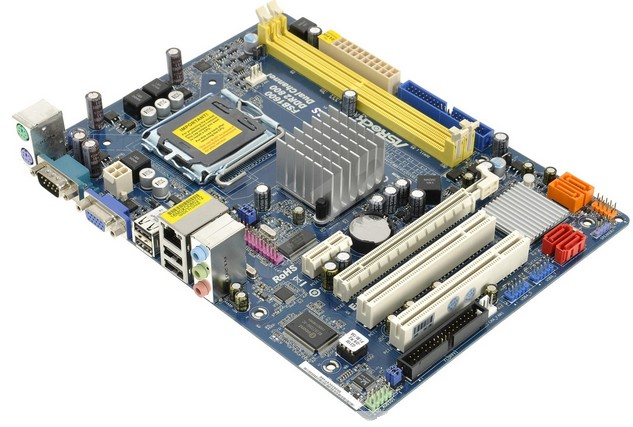
\includegraphics[width=0.8\textwidth]{fig/motherboard.jpg}
\end{center}

\end{frame}

\begin{frame}
\frametitle{What is Inside Computer}

Disassembled mobile phone:
\begin{center}
   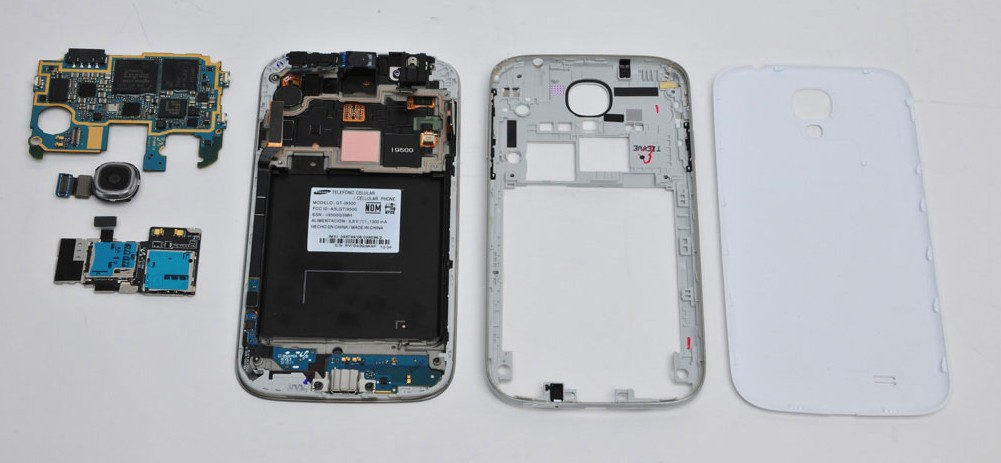
\includegraphics[width=0.6\textwidth]{fig/mobile.jpg}
\end{center}
\begin{center}
   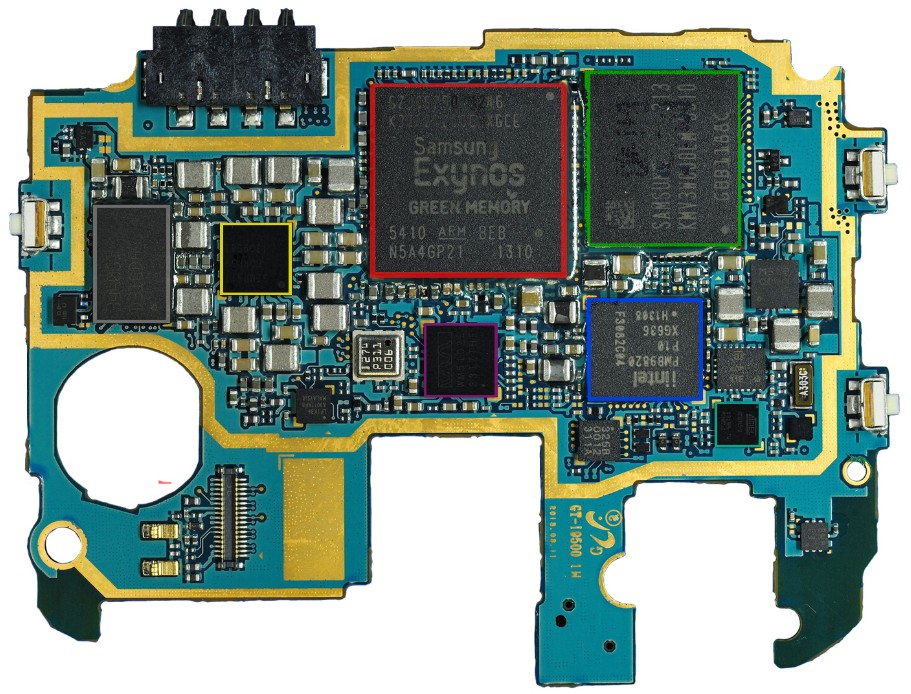
\includegraphics[width=0.4\textwidth]{fig/mobile-cpu.jpg}
\end{center}
\end{frame}


\begin{frame}
\frametitle{von Neumann}

The general computer concept presented by Johnem von Neumannem (1903-1957), Hungarian-American mathematician, physicist:
\begin{itemize}
\item Processor - Central Processing Unit - CPU
\item Memory, Random-access Memory
\item Input/Output
\end{itemize}
\begin{center}
   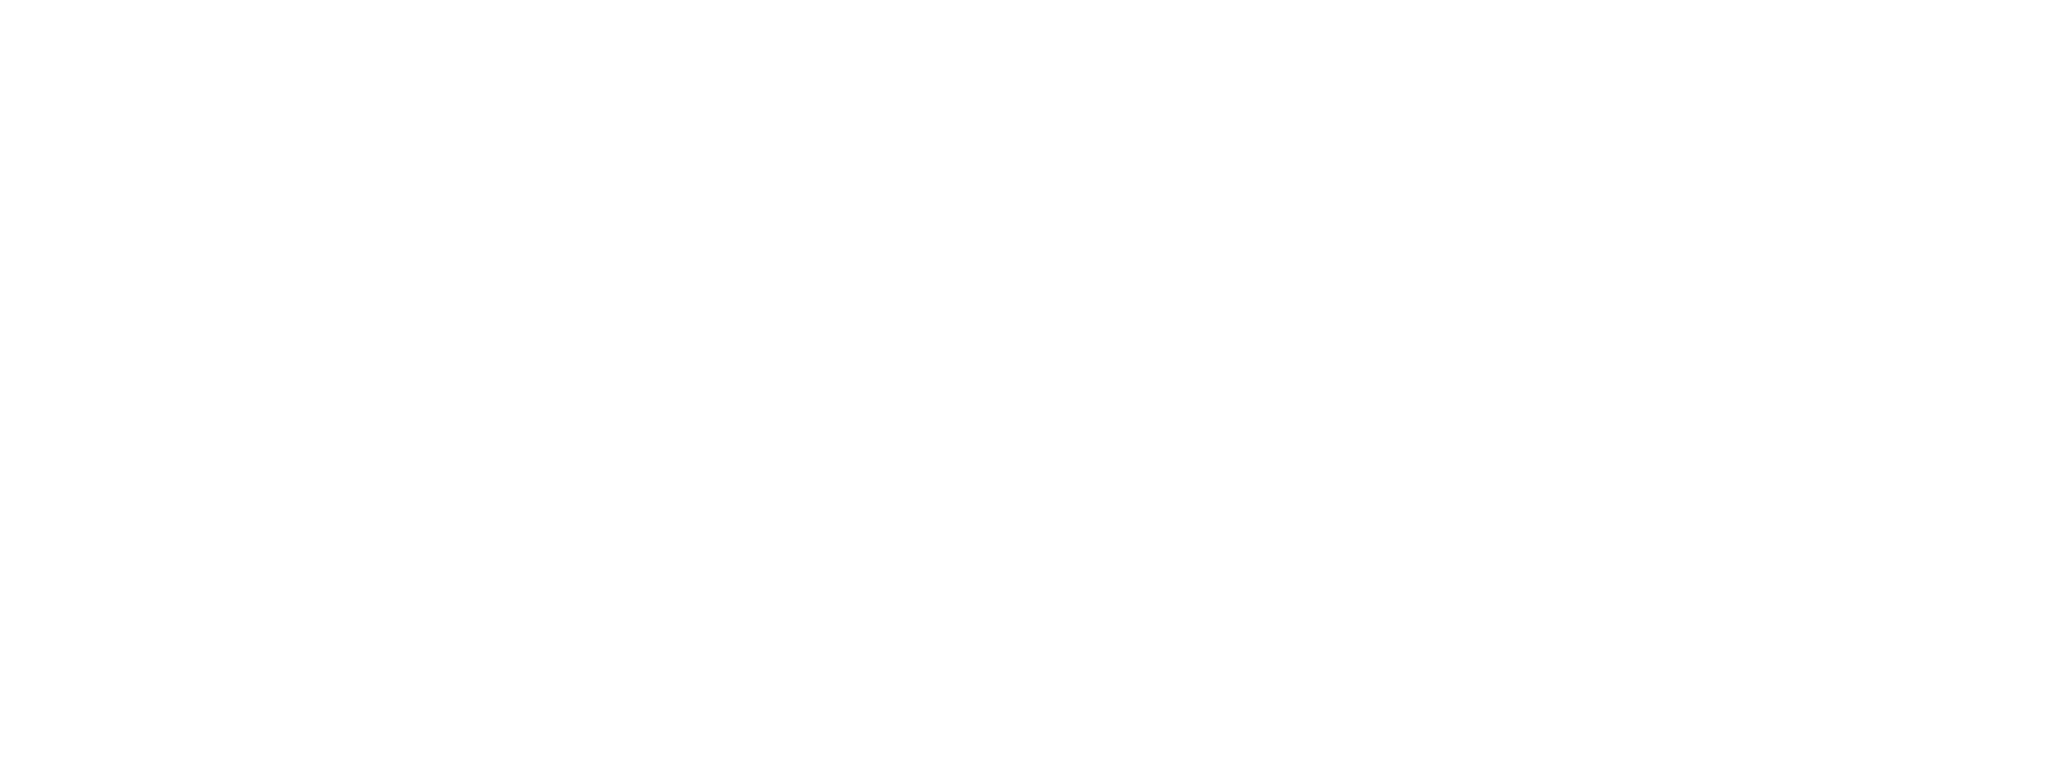
\includegraphics[width=0.7\textwidth]{cpu-vonNeumann.pdf}
\end{center}

\end{frame}


\begin{frame}
\frametitle{CPU -- Central Processing Unit}
\begin{columns}
\begin{column}{0.50\textwidth}
\begin{itemize}
\item General purpose (user/integer) registers (GPRs) -- usually 8, 16, 32 or 64-bits wide according to CPU architecture
\item CPU fetches instructions from the memory (basically in order) and executes each fetched and decoded instruction
\end{itemize}
\end{column}
\begin{column}{0.50\textwidth}  
\begin{center}
   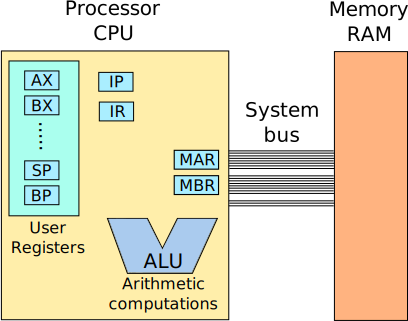
\includegraphics[width=0.95\textwidth]{cpu-en.pdf}
\end{center}
\end{column}
\end{columns}
\begin{itemize}
\item PC (program counter) or IP (instruction pointer) -- special register holding address of the instruction to be executed
\item ALU (arithmetic-logic unit) -- CPU component which proceed add, subtract, multiply, divide and other arithmetic and logical operations
\end{itemize}

\end{frame}



\begin{frame}
\frametitle{Main Memory}

Memory holds data values - bytes, words.

If you already know some programming language, then you can consider memory as array of same sized elements, i.e.\ for C-language:\\
\texttt{unsigned char RAM[16 * 1024 * 1024 *1024]; // 16GiB RAM}

\bigskip
The memory allows to read from specified location (address):\\
\texttt{register R10 = RAM[address];}\\
and write to specified address (source/target is usually one of GPRs):\\
\texttt{RAM[address] = R10;}
\bigskip

Address is numeric index into array which is usually encoded/transferred in binary representation on the signals connecting CPU to the memory

\end{frame}

\begin{frame}
\frametitle{Processor Instructions}

\begin{itemize}
\item The instructions encode all (limited set of operations) that the processor can perform
\item The basic instructions are:
\begin{itemize}
\item store a constant in the register
\item load data from memory into the register
\item perform a mathematical operation on the registers and store the result in the register
\item store data from the register in memory
\item compare two numbers
\item perform other instructions according to the result of the comparison (change the PC to a value other than the following instruction = perform a jump or branch in the program)
\end{itemize}
\item all programs, whether created in C language, Python, even programs performing very complex calculations are realized (compiled into) these simple processor instructions or interpreted by program written in these instructions
\end{itemize}

\end{frame}

\begin{frame}
\frametitle{Processor Instructions -- Instruction Set Architecture}

Instruction Set Architecture (ISA)
\begin{itemize}
\item  is a complete instruction set specification for given chip/architecture, defines address modes, data widths, operations, encoding
\item i.e.\ x86 (IA-32), x86-64 (AMD64, EM64T, IA-32e), ARM32, AArch64 (ARM64), AVR, MIPS, RISC-V
\item given ISA specifies:
\begin{itemize}
\item the list of known processor machine instruction set
\item supported data types, their widths and encoding (integers, signed integers, real/floating point numbers, vector types)
\item the set of user visible general purpose register, optionally floating point ones and special status and control ones
\item addressing modes (how the address to memory location can be formed)
\item memory organization (if byte accessible, word, halfword, etc.)
\end{itemize}
\end{itemize}

\end{frame}


\begin{frame}
\frametitle{Two Basic Concepts How to Architect ISA}

\begin{columns}
\begin{column}{0.5\textwidth}
\begin{center}
\LARGE{RISC}
\end{center}
Reduced Instruction Set Computer
\begin{itemize}
\item Usually a smaller number of instructions
\item All instructions have the same width and encoding rules (sometimes half-length aliases for denser encoding)
\item Fewer instructions and simpler addressing modes
\item Mathematical operations ALU only within registers (i.e.,\ load-store architecture)
\end{itemize}
\end{column}
\begin{column}{0.5\textwidth}  
\begin{center}
\LARGE{CISC}
\end{center}
Complex Instruction Set Computer
\begin{itemize}
\item Usually a larger number of instructions
\item The length of instructions even from 1 byte to e.g.\ 14 bytes, the most common instructions are the shortest
\item Usually many complex addressing modes
\item Data processing operations (ALU) even with values read/written to memory
\end{itemize}

\end{column}
\end{columns}
\end{frame}


\begin{frame}
\frametitle{Higher Level Program to Machine Level Compilation}

How come you have not heard about machine instructions yet?

\begin{center}
   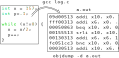
\includegraphics[width=0.65\textwidth]{preklad.pdf}
\end{center}

\begin{itemize}
\item Programming in assembler (assembly language) is often inefficient, hard, takes a long time and application is fixed to one ISA.
\item Compiler translates higher programming language directly into machine instructions of the target processor
\item Cross-compilation -- program translation for a different processor ISA than is used on machine to compile program
\end{itemize}
\end{frame}



\begin{frame}
\frametitle{Processor -- Hardware Implementation}

What does a processor consist of (physically)?

\begin{itemize}
\item You may have heard that a processor contains, say, 16 billion transistors
\item In 1965, Intel co-founder Gordon Moor formulated a law:
\begin{itemize}
\item The number of transistors that can be placed on an integrated circuit doubles every 18 months or so, at the same price.
\end{itemize}
\item More or less holds true until today, even though we are getting to the limits of physical possibilities.
\end{itemize}

Why do we need transistors in a processor (CPU)?
\begin{itemize}
\item To implement the Boolean algebra and registers (combinational and sequential logic).
\end{itemize}
We often can focus on block building system at given level of hierarchy, i.e.,\ ISA, register transfer level RTL, logic functions, gates, transistors, semiconductor/silicon structures, atomic-gratings
\end{frame}



\section{Boolean Algebra}



\begin{frame}
\frametitle{Boolean Algebra -- Values and Operations}

Boolean algebra is mathematical structure (see group theory):
\begin{itemize}
\item Only two values (states) for variables are allowed (0 and 1)
\begin{itemize}
\item 0/1, or False/True, or indicator/LED is on or off, or voltage representation 0V/5V
\end{itemize}
\item Addition operation (or, ||, $\lor$)
\begin{itemize}
\item 0+0=0 \phantom{XXXX}  0+1=1
\item 1+0=1 \phantom{XXXX}  1+1=1
\end{itemize}
\item Multiplication operation (and, \&\&, $\land$)
\begin{itemize}
\item 0*0=0 \phantom{XXXX}  0*1=0
\item 1*0=0 \phantom{XXXX}  1*1=1
\end{itemize}
\item Inversion, complementary element (negation, !, not, $\neg$)
\begin{itemize}
\item -0 = 1
\item -1 = 0
\end{itemize}
\end{itemize}
\end{frame}


\begin{frame}
\frametitle{Boolean Algebra -- States Representation}

Boolean algebra can be implemented well with voltages and transistors

\begin{columns}
\begin{column}{0.45\textwidth}
The voltage of a single conductor/signal to the ground defines a boolean value.
\end{column}
\begin{column}{0.55\textwidth}
\begin{center}
   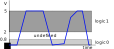
\includegraphics[width=0.9\textwidth]{ttl_log01-en.pdf}
\end{center}
\end{column}
\end{columns}

\begin{columns}
\begin{column}{0.45\textwidth}
Example: A boolean not operation, one X input conductor, one Y output conductor.
\end{column}
\begin{column}{0.55\textwidth}  
\begin{center}
   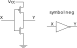
\includegraphics[width=0.8\textwidth]{cmos_neg.pdf}
\end{center}
\end{column}
\end{columns}

%inkscape ctrl shift Y logic symbols
\end{frame}

\begin{frame}
\frametitle{Boolean Algebra -- NAND, NOR, XOR}

Extended set of binary operations \texttt{nand}, \texttt{nor}, \texttt{xor} which can be decomposed to basic operations (this holds for circuit of arbitrary complexity) (\texttt{and}, \texttt{or}, \texttt{not}):

\begin{tabular}{ll}
\texttt{X nand Y} & \texttt{= not(X and Y)}\\
\texttt{X nor Y} & \texttt{= not(X or Y)}\\
\texttt{X xor Y} & \texttt{= (X or Y) and (not(X and Y))}\\
& \texttt{= (X or Y) and (X nand Y)}\\
\end{tabular}


\end{frame}


\begin{frame}
\frametitle{Boolean Algebra -- Logic Gates and Symbols}

List of the logic gates and their symbols for binary operations
\begin{center}
   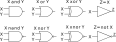
\includegraphics[width=0.8\textwidth]{log_symbols.pdf}
\end{center}

Summary table of basic logic gates:
\begin{tabular}{|c|c|c|c|c|c|c|c|}\hline
X & Y & X and Y & X or Y & X xor Y & X nand Y & X nor Y & X xnor Y \\\hline
0 & 0 &    0    &   0    &    0    &     1    &    1    &    1     \\\hline
0 & 1 &    0    &   1    &    1    &     1    &    0    &    0     \\\hline
1 & 0 &    0    &   1    &    1    &     1    &    0    &    0     \\\hline
1 & 1 &    1    &   1    &    0    &     0    &    0    &    1     \\\hline
\end{tabular}

\end{frame}


\begin{frame}
\frametitle{Boolean Algebra -- Quiz 1}

Signals/wires can also branch. What does the following circuit do?
\begin{center}
   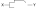
\includegraphics[width=0.4\textwidth]{not_jako_nand.pdf}
\end{center}

\begin{tabular}{ll}
A) it can't be connected like this \phantom{XXXX} & B) the result is X and Y\\
C) the result is X and not Y                     & D) the result is not X
\end{tabular}

\end{frame}


\begin{frame}
\frametitle{Logic/Combinational Circuits -- Quiz 2}

Some functions can be converted to gates even more efficiently than via the basic logic functions and, or, not.

The nand gate is the basic gate and all other gates can be built from it.

\begin{center}
   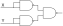
\includegraphics[width=0.5\textwidth]{or_by_nand.pdf}
\end{center}

Quiz: What is the result function equivalent to:
\begin{itemize}
\item[A] X and Y
\item[B] X or Y
\item[C] X xor Y
\item[D] X nor Y
\end{itemize}

\end{frame}


\begin{frame}
\frametitle{Logic/Combinational Circuits -- Quiz 3}

\begin{columns}
\begin{column}{0.55\textwidth}

More complex circuits can be made up of basic logical elements - gates. The signals can branch, they are combined together by some logical operation. The result is always only the logical values 0 or 1.

\bigskip

Quiz: What is the circuit function:
\begin{itemize}
\item[A] Nothing reasonable, it is just a tangle of wires
\item[B] It is a multiplexor, the value Z is one of the signals X according to the encoded value at Y
\item[C] It is a divider, the value Z is X/Y
\item[D] The value Z is 1 if X > Y
\end{itemize}
\end{column}
\begin{column}{0.45\textwidth}
\begin{center}
   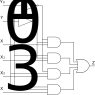
\includegraphics[width=0.95\textwidth]{multiplex.pdf}
\end{center}
\end{column}
\end{columns}


\end{frame}


\begin{frame}
\frametitle{Binary Encoding/Representation/Numeral System -- Quiz 4}

Quiz: One wire represents one value, either 0 or 1. How to represent more values/symbols, like all integers from 0 to 255 (i.e.,\ one byte)?
\begin{itemize}
\item[A] One wire has 8 different voltage levels
\item[B] One wire represents 8 different 0/1 values consecutively over time
\item[C] Eight wires, each representing one of the 0/1 values at one time
\item[D] 256 wires, only one has a value of 1
\end{itemize}

\end{frame}


\begin{frame}
\frametitle{Binary/Base-2 Numeral System}

Numbers represented by more digits or bits -- numeral system

Especially in the case of binary encoding

\begin{itemize}
\item multiple single-bit parallel conductors/wires/signals
\begin{itemize}
\item usually 8, 16, 32, 64 (powers of 2)
\item sometimes only parts of word is enough, like 5-bit (32 values)
\end{itemize}
\item order of conductors is important
\begin{itemize}
\item each conductor represents value at given power of 2
\item conductor $a_{i}$, total value $s = \sum_{i=0}^{63} a_{i}*2^{i}$
\end{itemize}
\end{itemize}

\end{frame}

\section{Arithmetic Adders}

\begin{frame}
\frametitle{Addition -- Two Single Bit Values}

Addition of two single bit numbers:
\begin{tabular}{|r|r|c|}\hline
X & Y & X+Y\\ \hline
0 & 0 & 00\\ \hline
0 & 1 & 01\\ \hline
1 & 0 & 01\\ \hline
1 & 1 & 10\\ \hline
\end{tabular}

\bigskip

\begin{columns}
\begin{column}{0.55\textwidth}
The result of the arithmetic sum fits into two bits, $C$ -- carry, $S$ -- sum.
\bigskip

\texttt{$S$ = $X$ xor $Y$}\\
\texttt{$C$ = $X$ and $Y$}

\bigskip

This logic circuit is called a Half Adder.
\end{column}
\begin{column}{0.45\textwidth}  
\begin{center}
   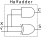
\includegraphics[width=0.75\textwidth]{half_adder.pdf}
\end{center}
\end{column}
\end{columns}

\end{frame}

\begin{frame}
\frametitle{Addition -- Full Adder}

If we add multi-bit numbers, we need to add three bit inputs later.

\begin{columns}
\begin{column}{0.6\textwidth}
The result of the sum is again a two-bit number: $C_{out}$~-~carry, $S$~-~sum.

\begin{columns}
\begin{column}{0.55\textwidth}

\bigskip

\begin{tabular}{|r|r|r|c|}\hline
C & X & Y & C+X+Y\\ \hline
0 & 0 & 0 & 00\\ \hline
0 & 0 & 1 & 01\\ \hline
0 & 1 & 0 & 01\\ \hline
0 & 1 & 1 & 10\\ \hline
1 & 0 & 0 & 01\\ \hline
1 & 0 & 1 & 10\\ \hline
1 & 1 & 0 & 10\\ \hline
1 & 1 & 1 & 11\\ \hline
\end{tabular}

\end{column}
\begin{column}{0.45\textwidth}

\texttt{$S_1$ = ($X$ xor $Y$)}\\
\texttt{$S$ = ($S_1$ xor $C$)}\\
\texttt{$C_1$ = ($X$ and $Y$)}\\
\texttt{$C_2$ = ($S_1$ and $C$)}\\
\texttt{$C_{out}$ = $C_1$ or $C_2$}

\bigskip

This logic circuit is called a full adder.

(Full adder)
\end{column}
\end{columns}

\end{column}
\begin{column}{0.4\textwidth}  

\begin{center}
   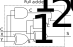
\includegraphics[width=\textwidth]{full_adder.pdf}
\end{center}


\begin{center}
   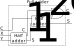
\includegraphics[width=\textwidth]{full_adder2.pdf}
\end{center}

\end{column}
\end{columns}


\end{frame}

\begin{frame}
\frametitle{Addition -- Ripple Carry Adder}

The simplest multi-bit asthmatics adder is built by connection of one half adder and multiple full adders.

This type of adder is called Ripple Carry Adder (chained full-adders).

\begin{center}
   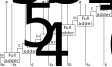
\includegraphics[width=0.7\textwidth]{ripple_adder.pdf}
\end{center}

$a_5a_4a_3a_2a_1a_0 + b_5b_4b_3b_2b_1b_0 = s_6s_5s_4s_3s_2s_1s_0$ where $s_6 = c_6$

\end{frame}

\begin{frame}
\frametitle{Addition -- Ripple Carry Adder}

What is the speed of Ripple Carry Adder?
\begin{itemize}
\item If the signal propagation delay of one gate is N, then the delay of Ripple Carry Adder for two 64-bit values is 63*2*N+N
\item Is this important?
\begin{itemize}
\item Yes, consider CPU clock 4GHz, one clock cycle takes 250\,ps (picosecond)
\item The limit is even speed of the signal propagation (< light speed) 0.3\,mm/ps, it is maximal speed of information propagation
\item When about 10\,ps gate propagation time is considered then Ripple Carray Adder adds 2 64-bit values in 1270\,ps (that is more than 5 clock cycles -- today ALU instruction latency is usually one cycle).
\end{itemize}
\item Is the faster implementation possible?
\begin{itemize}
\item Yes, Carry Lookahead Adder (CLA)
\end{itemize}
\end{itemize}

\end{frame}

\begin{frame}
\frametitle{Addition -- Carry Lookahead Adder}

\begin{itemize}
\item Is it possible to determine $C_1$, $C_2$, ... , directly form the addends?
\begin{itemize}
\item Yes, but for longer inputs it is expensive, requires large gates count.
\item The following example consider 4-bit inputs
\item We can define two basic functions:
\begin{itemize}
\item Carry generate -- case $A_i=1$ and $B_i=1$ implicates $C_{i+1}=1$ -- carry is generated $G_i=A_i \land B_i$ 
\item carry propagate -- case $A_i=1$ or $B_i=1$ implicates $C_{i+1}=C_{i}$ -- carry will be propagated, of there is carry in the lower bit; $P_i=A_i$ xor $B_i$ 
\end{itemize}
\item For 4-bit input:
\begin{itemize}
\item $C_1=G_0$ 
\item $C_2=G_1 \lor (C_1 \land P_1)= G_1 \lor (G_0 \land P_1)$
\item $C_3=G_2 \lor (C_2 \land P_2)= G_2 \lor (G_1 \land P_2) \lor (G_0 \land P_1 \land P_2)$ 
\item $C_4=G_3 \lor (C_3 \land P_3)= G_3 \lor (G_2 \land P_3) \lor (G_1 \land P_2 \land P_3) \lor (G_0 \land P_1 \land P_2 \land P_3)$
\item it is easy to extend expression for higher order bit, but it spans longer and longer
\end{itemize}
\end{itemize}
\end{itemize}

\end{frame}

\begin{frame}
\frametitle{Addition -- Carry Lookahead Adder}

The adder sums two 4-bit inputs in the time equivalent to propagation delay on four (4) serial connected gates.

\begin{center}
   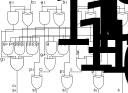
\includegraphics[width=0.65\textwidth]{lookahead_direct.pdf}
\end{center}

But for two 64-bit inputs, the adder would require $10^{20}$ gates to be built.
\end{frame}



\begin{frame}
\frametitle{Addition -- Carry Lookahead Adder}

How to resolve reasonably fast function for larger numbers, i.e., 64-bit?

\begin{columns}
\begin{column}{0.45\textwidth}
\begin{itemize}
\item The 4-bit adder is extended to allow $C$ input from lower order bits
\begin{itemize}
\item WARNING some gates has to be added
\end{itemize}
\item We can chain these adder blocks.
\end{itemize}
\end{column}
\begin{column}{0.55\textwidth}
\begin{center}
   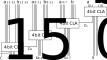
\includegraphics[width=0.95\textwidth]{lookahead_ripple.pdf}
\end{center}
\end{column}
\end{columns}


\begin{itemize}
\item The latency/delay of 16-bit adder (in the figure) is 16 gate delays
\item The latency/delay of 64-bit adder is 64 gate delays, much better than 127 gate delays for simple Ripple Carry Adder.
\end{itemize}

\end{frame}


\begin{frame}
\frametitle{Addition -- Carry Select Adder}

\begin{itemize}
\item It is certain that Carry is 0 or 1
\item 4-bit CLA can be doubled and the result is computed for both Carry inputs 0 and 1 in parallel
\item Only the multiplexer control is chained which chooses result accordingly if to Carry is 0 or 1
\end{itemize}
\begin{center}
   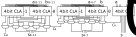
\includegraphics[width=0.75\textwidth]{lookahead_select.pdf}
\end{center}

\begin{itemize}
\item The adder is faster, instead of delay 4 gates will chain only delay 2 gates for multiplexer
\item The speed of the 16-bit adder from the figure will be 10 gate delays
\item The speed of the 64-bit adder will be 34 gate delays, which is slightly better than the 64 delay for CLA chaining.
\end{itemize}

\end{frame}


\begin{frame}
\frametitle{Addition -- Carry Lookahead Adder, Block Version}

Yet another attempt to speed up adder
\begin{itemize}
\item The carry generate and propagate operation can be defined for larger groups of bits:
\begin{itemize}
\item If orders from $i$ to $j$ generate carry, then $G_{i,j}=1$
\item If orders from $i$ to $j$ propagate carry, then $P_{i,j}=1$
\end{itemize}
\item Following rules are defined, how to compute $G_{i,k}$ and $P_{i,k}$ based on $G_{i,j}$, $G_{j+1,k}$,$P_{i,j}$, $P_{j+1,k}$
\begin{itemize}
\item $G_{i,k}=G_{j+1,k} \lor (G_{i,j} \land P_{j+1,k})$
\item $P_{i,k}=P_{i,j} \land P_{j+1,k}$
\end{itemize}
\item The initial values are old known $G_i$ and $P_i$. 
\item That is $G_{i,i}=G_i=a_i \land b_i$ and $P_{i,i}=P_i=a_i$ xor $b_i$.
\end{itemize}

\end{frame}

\begin{frame}
\frametitle{Addition -- Carry Lookahead Adder, Block Gen. and Prop.}

The computation of the previously defined rules can be realized as:
\begin{columns}
\begin{column}{0.55\textwidth}
\begin{center}
   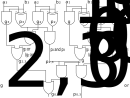
\includegraphics[width=0.95\textwidth]{lookahead_tree.pdf}
\end{center}
\end{column}
\begin{column}{0.45\textwidth}

The time co compute pair $G_{i,k}$ and $P_{i,k}$:
\begin{itemize}
\item Delay for 4-bit addends -- 5\,gate delays
\item Delay for 8-bit addends -- 7\,gate delays
\item Delay for 16-bit addends -- 9\,gate delays
\item Delay for 32-bit addends -- 11\,gate delays
\item Delay for 64-bit addends -- 13\,gate delays
\end{itemize}

\end{column}
\end{columns}

\end{frame}

\begin{frame}
\frametitle{Addition -- Carry Lookahead Adder, Example}

Evaluation of carry generate and propagate block with use of:
\begin{itemize}
\item $g_h$, $p_h$ -- generate and propagate carry in higher (more significant) subblock
\item $g_l$, $p_l$ -- generate and propagate carry in lower (less significant) subblock
\end{itemize}
\begin{table}
\begin{tabular}{|c|c|c|c|c|c|c|c|c|}\hline
a & 0 & 0 & 1 & 0 & 1 & 0 & 0 & 1 \\ \hline
b & 1 & 0 & 1 & 1 & 0 & 1 & 1 & 1 \\ \hhline{|=|=|=|=|=|=|=|=|=|}
g = $a_i$ and $b_i$ & 0 & 0 & 1 & 0 & 0 & 0 & 0 & 1 \\ \hline
p = $a_i$ xor $b_i$ & 1 & 0 & 0 & 1 & 1 & 1 & 1 & 0 \\ \hhline{|=|=|=|=|=|=|=|=|=|}
g = $g_h$ or ( $g_l$ and $p_h$ )& \multicolumn{2}{c|} 0 & \multicolumn{2}{c|} 1 & \multicolumn{2}{c|} 0 & \multicolumn{2}{c|} 1 \\ \hline
p = $p_h$ and $p_l$ & \multicolumn{2}{c|} 0 & \multicolumn{2}{c|} 0 & \multicolumn{2}{c|} 1 & \multicolumn{2}{c|} 0 \\ \hhline{|=|==|==|==|==|}
g = $g_h$ or ( $g_l$ and $p_h$ ) & \multicolumn{4}{c|} 0 & \multicolumn{4}{c|} 1  \\ \hline
p = $p_h$ and $p_l$ & \multicolumn{4}{c|} 0 & \multicolumn{4}{c|} 0  \\ \hhline{|=|====|====|}
g = $g_h$ or ( $g_l$ and $p_h$ ) & \multicolumn{8}{c|} 0   \\ \hline
p = $p_h$ and $p_l$ & \multicolumn{8}{c|} 0   \\ \hline
\end{tabular}
\end{table}
\end{frame}

\begin{frame}
\frametitle{Addition -- Carry Lookahead Adder, Hierarchy}

It is necessary to compute all Carry $C_i$, in the case of hypothetical chaining we know $C_0$, if not then:
\begin{itemize}
\item We use tree hierarchy again but in the reversed order of computation $P_{i,j}$ and $G_{i,j}$:
\begin{itemize}
\item If we know $C_i$, $G_{i,j}$ and $P_{i,j}$
\item then $C_{j+1} = G_{i,j} \lor (C_i \land P_{i,j})$ 
\end{itemize}
\item The evaluation for 4-bit adder will be processed in the next specified order:
\begin{itemize}
\item $C_4 = G_{0,3} \lor (C_0 \land P_{0,3})$, $C_2 = G_{0,1} \lor (C_0 \land P_{0,1})$
\item $C_3 = G_{2,2} \lor (C_2 \land P_{2,2})$, $C_1 = G_{0,0} \lor (C_0 \land P_{0,0})$
\end{itemize}
\item The delay for $2\times$ wider inputs (addends) increases by 2 gates delays 
\item For 64-bit addends, the time required to compute all $C_i$ is 12 gates delays.
\item The complete addition for 64-bit inputs takes 26 gates delays.
\end{itemize}

\end{frame}


\begin{frame}
\frametitle{Addition - Carry Lookahead Adder, Final Sum}

The evaluation of $C_i$ then can be seen from:
\begin{columns}
\begin{column}{0.5\textwidth}
\begin{center}
   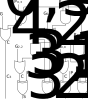
\includegraphics[width=0.95\textwidth]{lookahead_tree_carry.pdf}
\end{center}
\end{column}
\begin{column}{0.5\textwidth}

The time to evaluate $G_{i,k}$ pairs $P_{i,k}$:
\begin{itemize}
\item Delay for 4-bit addends is 5 gate delays
\item Delay for 8-bit addends is 7 gate delays
\item Delay for 64-bit addends is 13 gate delays
\end{itemize}

\end{column}
\end{columns}

\end{frame}


\begin{frame}{shrink=5}
\frametitle{Addition -- Carry Lookahead Adder, Example}

The carry is evaluated from less significant blocks and g, p expressions:
\begin{itemize}
\item $C_i = g$ or $(p$ and $C_{i-k})$ -- carry prop. or gen. from lower orders
\end{itemize}
\begin{table}
\footnotesize
\begin{tabular}{|p{0.02\textwidth}|p{0.08\textwidth}|p{0.08\textwidth}|p{0.08\textwidth}|p{0.08\textwidth}|p{0.08\textwidth}|p{0.08\textwidth}|p{0.08\textwidth}|p{0.08\textwidth}|}\hline
a & 0 & 0 & 1 & 0 & 1 & 0 & 0 & 1 \\ \hline
b & 1 & 0 & 1 & 1 & 0 & 1 & 1 & 1 \\ \hhline{|=|=|=|=|=|=|=|=|=|}
g  & 0 & 0 & 1 & 0 & 0 & 0  & 0 & 1 \\ \hline
p & 1 & 0 & 0 & 1   & 1 & 1 & 1 & 0 \\ \hline
C & \multicolumn{2}{p{0.16\textwidth}|}{}  & \multicolumn{2}{p{0.16\textwidth}|}{} & \multicolumn{2}{p{0.16\textwidth}|}{} & \multicolumn{2}{p{0.16\textwidth}|}{}  \\ \hhline{|=|=|=|=|=|=|=|=|=|}
g & \multicolumn{2}{c|} 0 & \multicolumn{2}{c|}{\textcolor{brown}1} & \multicolumn{2}{c|} 0 & \multicolumn{2}{c|} 1 \\ \hline
p  & \multicolumn{2}{c|} 0 & \multicolumn{2}{c|}{\textcolor{teal} 0} & \multicolumn{2}{c|} 1 & \multicolumn{2}{c|} 0 \\ \hline
C  & \multicolumn{2}{l|}{} & \multicolumn{2}{l|}{} & \multicolumn{2}{l|}{} & \multicolumn{2}{l|}{} \\ \hhline{|=|==|==|==|==|}
g  & \multicolumn{4}{c|} 0 & \multicolumn{4}{c|}{\textcolor{cyan}1}  \\ \hline
p  & \multicolumn{4}{c|} 0 & \multicolumn{4}{c|}{\textcolor{green}0}  \\ \hline
C  & \multicolumn{3}{c|}{} & \multicolumn{5}{l|}{$C_4$ = \textcolor{cyan}1 or ( \textcolor{green}0 and $C_0$) = 1}  \\ \hhline{|=|====|====|}
g  & \multicolumn{8}{c|} 0   \\ \hline
p  & \multicolumn{8}{c|} 0   \\ \hline
C  & \multicolumn{8}{l|}{$C_8$ = 0 or ( 0 and $C_0$) = 0}   \\ \hline
\end{tabular}
\end{table}
\end{frame}


\begin{frame}{shrink=5}
\frametitle{Addition -- Carry Lookahead Adder, Example}

The carry is evaluated from less significant blocks and g, p expressions:
\begin{itemize}
\item $C_i = g$ or $(p$ and $C_{i-k})$ -- carry prop. or gen. from lower orders
\end{itemize}
\begin{table}
\footnotesize
\begin{tabular}{|p{0.02\textwidth}|p{0.08\textwidth}|p{0.08\textwidth}|p{0.08\textwidth}|p{0.08\textwidth}|p{0.08\textwidth}|p{0.08\textwidth}|p{0.08\textwidth}|p{0.08\textwidth}|}\hline
a & 0 & 0 & 1 & 0 & 1 & 0 & 0 & 1 \\ \hline
b & 1 & 0 & 1 & 1 & 0 & 1 & 1 & 1 \\ \hhline{|=|=|=|=|=|=|=|=|=|}
g  & 0 & 0 & 1 & 0 & 0 & 0  & 0 & 1 \\ \hline
p & 1 & 0 & 0 & 1   & 1 & 1 & 1 & 0 \\ \hline
C & \multicolumn{2}{p{0.16\textwidth}|}{}  & \multicolumn{2}{p{0.16\textwidth}|}{} & \multicolumn{2}{p{0.16\textwidth}|}{} & \multicolumn{2}{p{0.16\textwidth}|}{}  \\ \hhline{|=|=|=|=|=|=|=|=|=|}
g & \multicolumn{2}{c|} 0 & \multicolumn{2}{c|}{\textcolor{brown}1} & \multicolumn{2}{c|} 0 & \multicolumn{2}{c|} 1 \\ \hline
p  & \multicolumn{2}{c|} 0 & \multicolumn{2}{c|}{\textcolor{teal} 0} & \multicolumn{2}{c|} 1 & \multicolumn{2}{c|} 0 \\ \hline
C  &  & \multicolumn{3}{l|}{$C_6$ = \textcolor{brown}1 or ( \textcolor{teal}0 and $C_4$) = 1} &  & \multicolumn{3}{l|}{$C_2$ = 1 or ( 0 and $C_0$) = 1} \\ \hhline{|=|==|==|==|==|}
g  & \multicolumn{4}{c|} 0 & \multicolumn{4}{c|}{\textcolor{cyan}1}  \\ \hline
p  & \multicolumn{4}{c|} 0 & \multicolumn{4}{c|}{\textcolor{green}0}  \\ \hline
C  & \multicolumn{3}{c|}{} & \multicolumn{5}{l|}{$C_4$ = \textcolor{cyan}1 or ( \textcolor{green}0 and $C_0$) = 1}  \\ \hhline{|=|====|====|}
g  & \multicolumn{8}{c|} 0   \\ \hline
p  & \multicolumn{8}{c|} 0   \\ \hline
C  & \multicolumn{8}{l|}{$C_8$ = 0 or ( 0 and $C_0$) = 0}   \\ \hline
\end{tabular}
\end{table}
\end{frame}


\begin{frame}{shrink=5}
\frametitle{Addition -- Carry Lookahead Adder, Example}

The carry is evaluated from less significant blocks and g, p expressions:
\begin{itemize}
\item $C_i = g$ or $(p$ and $C_{i-k})$ -- carry prop. or gen. from lower orders
\end{itemize}
\begin{table}
\footnotesize
\begin{tabular}{|p{0.02\textwidth}|p{0.08\textwidth}|p{0.08\textwidth}|p{0.08\textwidth}|p{0.08\textwidth}|p{0.08\textwidth}|p{0.08\textwidth}|p{0.08\textwidth}|p{0.08\textwidth}|}\hline
a & 0 & 0 & 1 & 0 & 1 & 0 & 0 & 1 \\ \hline
b & 1 & 0 & 1 & 1 & 0 & 1 & 1 & 1 \\ \hhline{|=|=|=|=|=|=|=|=|=|}
g  & 0 & \textcolor{red}0 & 1 & \textcolor{magenta}0 & 0 & \textcolor{brown}0  & 0 & \textcolor{purple}1 \\ \hline
p & 1 & \textcolor{blue}0 & 0 & \textcolor{green}1   & 1 & \textcolor{orange}1 & 1 & \textcolor{teal}0 \\ \hline
C & \multicolumn{2}{p{0.16\textwidth}|}{$C_7$ = \textcolor{red}0 or ( \textcolor{blue}0 and $C_6$) = 0}  & \multicolumn{2}{p{0.16\textwidth}|}{$C_5$ = \textcolor{magenta}0 or ( \textcolor{green}1 and $C_4$) = 1} & \multicolumn{2}{p{0.16\textwidth}|}{$C_3$ = \textcolor{brown}0 or ( \textcolor{orange}1 and $C_2$) = 1} & \multicolumn{2}{p{0.16\textwidth}|}{$C_1$ = \textcolor{purple}1 or ( \textcolor{teal}0 and $C_0$) = 1}  \\ \hhline{|=|=|=|=|=|=|=|=|=|}
g & \multicolumn{2}{c|} 0 & \multicolumn{2}{c|}{\textcolor{brown}1} & \multicolumn{2}{c|} 0 & \multicolumn{2}{c|} 1 \\ \hline
p  & \multicolumn{2}{c|} 0 & \multicolumn{2}{c|}{\textcolor{teal} 0} & \multicolumn{2}{c|} 1 & \multicolumn{2}{c|} 0 \\ \hline
C  &  & \multicolumn{3}{l|}{$C_6$ = \textcolor{brown}1 or ( \textcolor{teal}0 and $C_4$) = 1} &  & \multicolumn{3}{l|}{$C_2$ = 1 or ( 0 and $C_0$) = 1} \\ \hhline{|=|==|==|==|==|}
g  & \multicolumn{4}{c|} 0 & \multicolumn{4}{c|}{\textcolor{cyan}1}  \\ \hline
p  & \multicolumn{4}{c|} 0 & \multicolumn{4}{c|}{\textcolor{green}0}  \\ \hline
C  & \multicolumn{3}{c|}{} & \multicolumn{5}{l|}{$C_4$ = \textcolor{cyan}1 or ( \textcolor{green}0 and $C_0$) = 1}  \\ \hhline{|=|====|====|}
g  & \multicolumn{8}{c|} 0   \\ \hline
p  & \multicolumn{8}{c|} 0   \\ \hline
C  & \multicolumn{8}{l|}{$C_8$ = 0 or ( 0 and $C_0$) = 0}   \\ \hline
\end{tabular}
\end{table}
\end{frame}


\begin{frame}
\frametitle{Multiplexor}

Similar approach (divide and conquer - create a tree structure) can be used in the multiplexor implementation:
\begin{columns}
\begin{column}{0.5\textwidth}
\begin{center}
   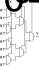
\includegraphics[width=0.5\textwidth]{multiplex-tree.pdf}
\end{center}
\end{column}
\begin{column}{0.5\textwidth}
\begin{itemize}
\item According to the three-bit number $x$ the corresponding input $a_x$ is selected for the output $Y$
\item It is not the fastest implementation, but it is clear
\item We can also use 4 input multiplex and reduce the number of tree levels.
\end{itemize}

\end{column}
\end{columns}

\end{frame}

\begin{frame}[fragile,shrink=5]
\frametitle{Bit Shift Operation}

\begin{itemize}
\item it is denoted in C-language by \texttt{>>} and \texttt{<<} operators
\begin{itemize}
\item The operations can be used for multiplication by power of two 2 -- operation \texttt{<<}; and for division by power of 2 -- operation \texttt{>>}
\end{itemize}
\item How to implement shift by k-bits?
\end{itemize}
\begin{columns}
\begin{column}{0.48\textwidth}
k-times rotate/shift by 1 bit\\
It can be compared to exponentiation algorithm:
\end{column}
\begin{column}{0.52\textwidth}
shift by 1, 2, 4, 8, 16 bits\\
Compare with fast exponentiation:
\end{column}
\end{columns}

\begin{columns}
\begin{column}{0.48\textwidth}
\begin{minted}{c}
double Exp(double a, int k) {
  if (k == 0) return 1;
  return a * Exp(a, k - 1);
}
\end{minted}
\end{column}
\begin{column}{0.52\textwidth}
\begin{minted}{c}
double FastExp(double a, int k) {
  if (k == 0) return 1;
  if (k % 2 == 0) {
    double i = FastExp(a, k / 2);
    return i * i;
  } else {
    return a * FastExp(a, k - 1);
  }
}
\end{minted}

\end{column}
\end{columns}



\end{frame}



\begin{frame}
\frametitle{Barrel Shifter}

Shift by 0-7 bits can be composed of shift by 1, 2, 4:
\begin{center}
   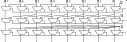
\includegraphics[width=0.75\textwidth]{barrel-shift.pdf}
\end{center}

\begin{itemize}
\item Multiplexor in each row selects identity operation (do nothing) or shifts by fixed number of bits
\item Single bit input signals $x_2,x_1,x_0$ are equivalent to binary representation of number of bits to shift
\item Example:
\begin{itemize}
\item shift by 5 bits is realized by serial combination of shift by 1 bit and shift by 4 bits ($x_2=1$, $x_1=0$, $x_0=1$)
\item shift by 3 bits is realized by serial combination of shift by 1 bit and shift by 2 bits ($x_2=0$, $x_1=1$, $x_0=1$)
\end{itemize}
\end{itemize}

\end{frame}


\begin{frame}
\frametitle{Quiz}

How many layers (row) a barrel shifter must have for 64-bit number, i.e.,\ for rotations from 0 to 63? (For rotations from 0 to 7, it was 3 layers)

\begin{itemize}
\item[A] 4
\item[B] 6
\item[C] 16
\item[D] 64
\end{itemize}

\end{frame}


\begin{frame}
\frametitle{Feedback Quiz}

How much did you understand today?
\begin{itemize}
\item[A] All without a problem.
\item[B] Almost everything.
\item[C] Almost nothing.
\item[D] Absolutely nothing.
\end{itemize}

\end{frame}


\end{document}

